%
% Layout retirado de http://www.di.uminho.pt/~prh/curplc09.html#notas
%
\documentclass{report}
\usepackage{graphicx}
\usepackage[portuguese]{babel}
\usepackage[utf8]{inputenc}
\usepackage{hyperref}
%\usepackage[latin1]{inputenc}
%\usepackage{url}
\usepackage{enumerate}
%\usepackage{alltt}
%\usepackage{fancyvrb}
%\usepackage{listings}
%LISTING - GENERAL
%\lstset{
%	basicstyle=\small,
%	numbers=left,
%	numberstyle=\tiny,
%	numbersep=5pt,
%	breaklines=true,
%    frame=tB,
%	mathescape=true,
%	escapeinside={(*@}{@*)}
%}

%\lstset{ %
%	language=Java,							% choose the language of the code
%	basicstyle=\ttfamily\footnotesize,		% the size of the fonts that are used for the code
%	keywordstyle=\bfseries,					% set the keyword style
%	%numbers=left,							% where to put the line-numbers
%	numberstyle=\scriptsize,				% the size of the fonts that are used for the line-numbers
%	stepnumber=2,							% the step between two line-numbers. If it's 1 each line
%											% will be numbered
%	numbersep=5pt,							% how far the line-numbers are from the code
%	backgroundcolor=\color{white},			% choose the background color. You must add \usepackage{color}
%	showspaces=false,						% show spaces adding particular underscores
%	showstringspaces=false,					% underline spaces within strings
%	showtabs=false,							% show tabs within strings adding particular underscores
%	frame=none,								% adds a frame around the code
%	%abovecaptionskip=-.8em,
%	%belowcaptionskip=.7em,
%	tabsize=2,								% sets default tabsize to 2 spaces
%	captionpos=b,							% sets the caption-position to bottom
%	breaklines=true,						% sets automatic line breaking
%	breakatwhitespace=false,				% sets if automatic breaks should only happen at whitespace
%	title=\lstname,							% show the filename of files included with \lstinputlisting;
%											% also try caption instead of title
%	escapeinside={\%*}{*)},					% if you want to add a comment within your code
%	morekeywords={*,...}					% if you want to add more keywords to the set
%}

\usepackage{xspace}

\parindent=0pt
\parskip=2pt

\setlength{\oddsidemargin}{-1cm}
\setlength{\textwidth}{18cm}
\setlength{\headsep}{-1cm}
\setlength{\textheight}{23cm}

\def\darius{\textsf{Darius}\xspace}
\def\antlr{\texttt{AnTLR}\xspace}
\def\pe{\emph{Publicação Eletrónica}\xspace}

\def\titulo#1{\section{#1}}
\def\super#1{{\em Supervisor: #1}\\ }
\def\area#1{{\em \'{A}rea: #1}\\[0.2cm]}
\def\resumo{\underline{Resumo}:\\ }


%%%%\input{LPgeneralDefintions}

\title{Processamento de Linguagens e Compiladores 3º ano\\ \textbf{Expressões Regulares e GAWK}\\ Grupo 14}
\author{Artur Queiroz\\ (A77136) \and  Rafael Fernandes\\ A78242 \and Rafaela Pinho\\ A77293  }
\date{\today}

\begin{document}

\maketitle

\begin{abstract}
Este trabalho foca os conceitos básicos do funcionamento GAWK e das expressões regulares utilizadas para descrever padrões.
Neste relatório descrevemos as decisões tomadas e as dificuldades encontradas, bem como pequenos exemplos para que qualquer um que o leia perceba facilmente como funciona o nosso projeto.
\end{abstract}

\tableofcontents

\chapter{Introdução} \label{intro}
Neste trabalho vamos filtrar vários ficheiros de internacionalização, utilizando expressões regulares e o sitema de filtragem de texto GAWK. Uma parte importante do sistema linux são as expressões regulares e a capacidade de procurar num input um determinado padrão, o que facilita muitas das operações
As expressões regulares são uma sequência de caracteres, sucinta e flexível, que identifica palavras ou pradrões de caracteres. Combinando-as com o sistema de filtragem, conseguimos extrair informações dos ficheiros POs que são documentos que contêm traduções de uma língua para outra.
Este trabalho tem como objetivos aprofundar os conhecimento do GAWK, do sistema Linux e as suas ferramentas, bem como aprender melhor o funcionamento das exprexões regulares.

%\section*{Estrutura do Relatório} \
%explicar como está organizado o documento, referindo os capítulos existentes em~\cite{Pereira201635}
%e a sua articulação explicando o conteúdo de cada um.
%No capítulo~\ref{fi} faz-se uma análise detalhada do problema proposto
%de modo a poder-se especificar  as entradas, resultados e formas de transformação.\\
%etc. \ldots\\
%No capítulo~\ref{concl} termina-se o relatório com uma síntese do que foi dito,
%as conclusões e o trabalho futuro

\chapter{Ficheiros de internacionalização} \label{fi}

\section{Descrição informal do problema}\
É necessária um "script" que permita:
\begin{enumerate}[a)]
\item Analisar vários ficheiros de formato PO, e devolver o número de traduções
e os seus tradutores, bem como alguns metadados acharmos relevantes.
\item Através de ficheiros PO's criar dicionários de triangulação de Português
para Francês.
\item Reformatar ficheiros de formato PO pra LaTeX.
\end{enumerate}

\section{Especificação do Requisitos}
Os requisitos mínimos deste tarbalho são saber utilizar Linux, bash e GAWK.

\chapter{Concepção/desenho da Resolução}
\section{Estruturas de Dados}
\section{Algoritmos}
Utilizamos as seguintes expressões regulares:

\begin{enumerate}[i)]
\item /\^{}msgid/
\item /\^{}"Language:/
\item /\textless.*@.*\textgreater/ \&\& !/\^{}"Report/ \&\& !/FIRST/ \&\& !/\^{}"Language/
\item /\^{}"Language-Team: *$\backslash$n"/
\item /\^{}"Language-Team:/
\item /portugu[êe]se?s?/
\item /\^{}msgid[ $\backslash$t]*""/
\item /\^{}msgstr[ $\backslash$t]*""/
\item /\^{}msgid *"/
\item /\^{}msgstr *"/
\end{enumerate}

\chapter{Codificação e Testes}
\section{Problemas de implementação, Decisões e Alternativas}
\subsection{Problemas de implementação}
De um modo geral no trabalho, tivemos problemas com a formatação de alguns ficheiros, dado não se encontrarem na formatação prevista, e com o LaTex.
\subsection{Decisões}
No problema 1 proposto no exercício, decidimos ignorar os "msgid" que não contivessem nenhuma mensagem ou que contivessem mais de uma tradução.Escolhemos como metadados mais importantes a linguagem, a percentagem de blocos, a quantidade de blocos por ficheiro, e quantos e quem são os tradutores. Decidimos também que a linguagem só está no "Language".
No problema 2 decidimos utilizar a "Language-team" para definir a linguagem de tradução, pois nenhum dos ficheiros apresentava linguagem no campo"Language". Usamos uma matriz descritiva, sendo as linhas a frase em inglês e os descritivos das colunas a linguagem portuguesa ou francesa. Assumimos só a linguagem portuguesa e a francesa e imprimimos unicamente o que tem tradução en triangulação.
No último problema ignoramos o "\\n" e o "\#", devido ao LaTex, sustituindo por "" e por --, respetivamente.
\subsection{Alternativas}
Uma alternativa seria modificar os ficheiros manualmente de modo a estarem no formato certo. Outra alternativa seria fazer inúmeros casos especiais.

\section{Testes realizados e Resultados}
Mostram-se a seguir alguns testes feitos (valores introduzidos) e
os respectivos resultados obtidos:


%\begin{figure}[h]
%\center
%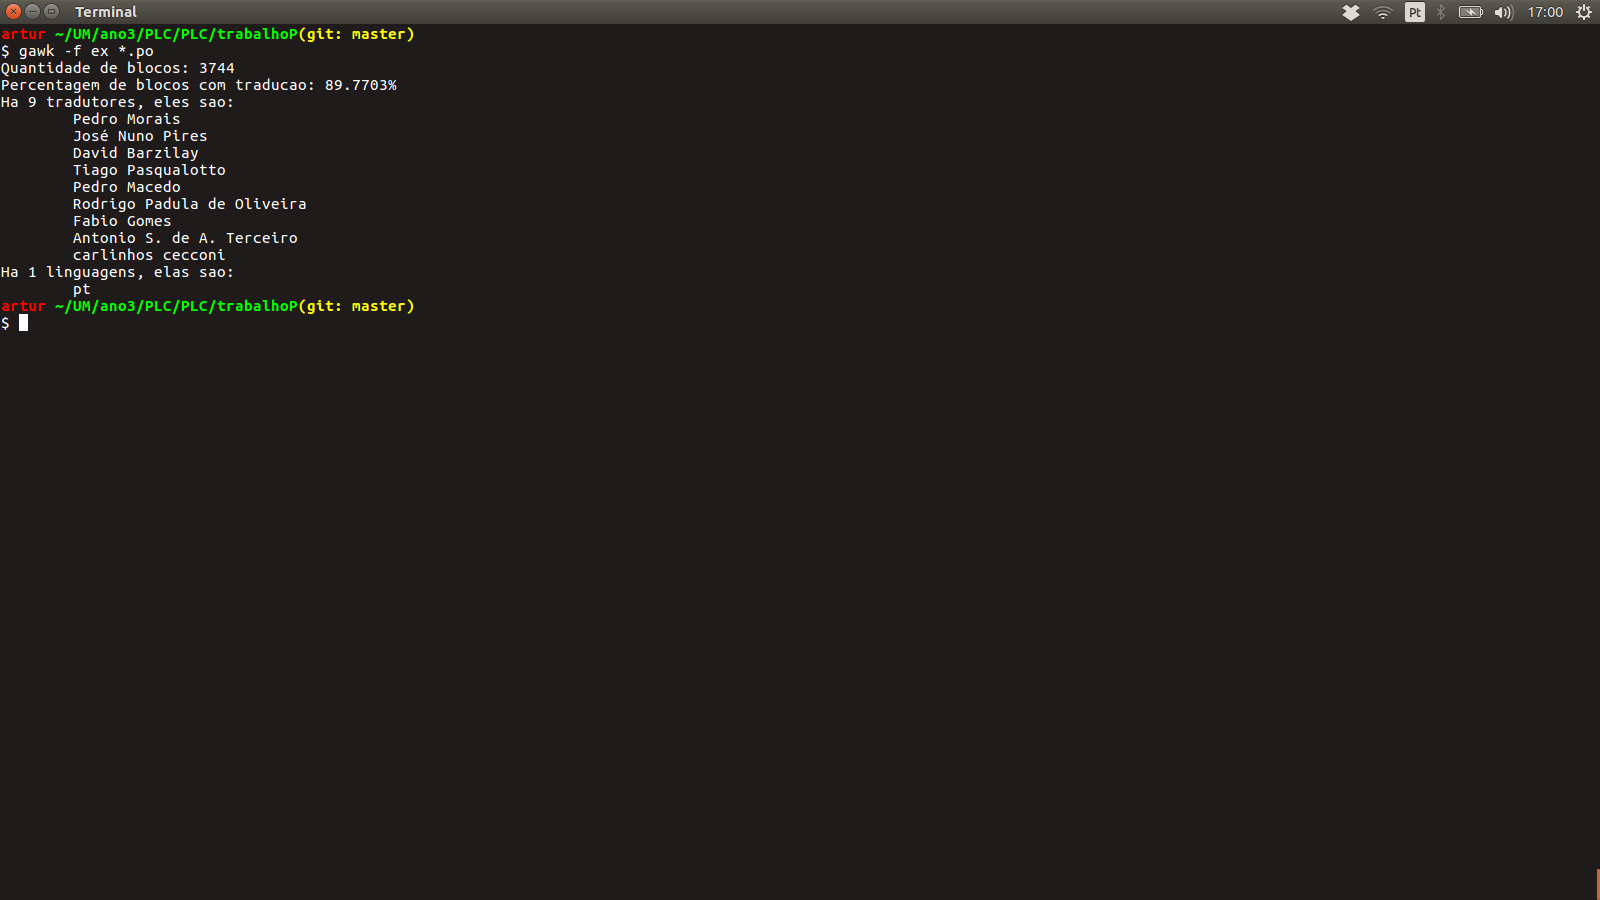
\includegraphics[scale=1]{exercicio1.png}
%\caption{Exercicio 1}
%\label{figura:Exercicio 1}
%\end{figure}

%\begin{figure}[h]
%\centering
%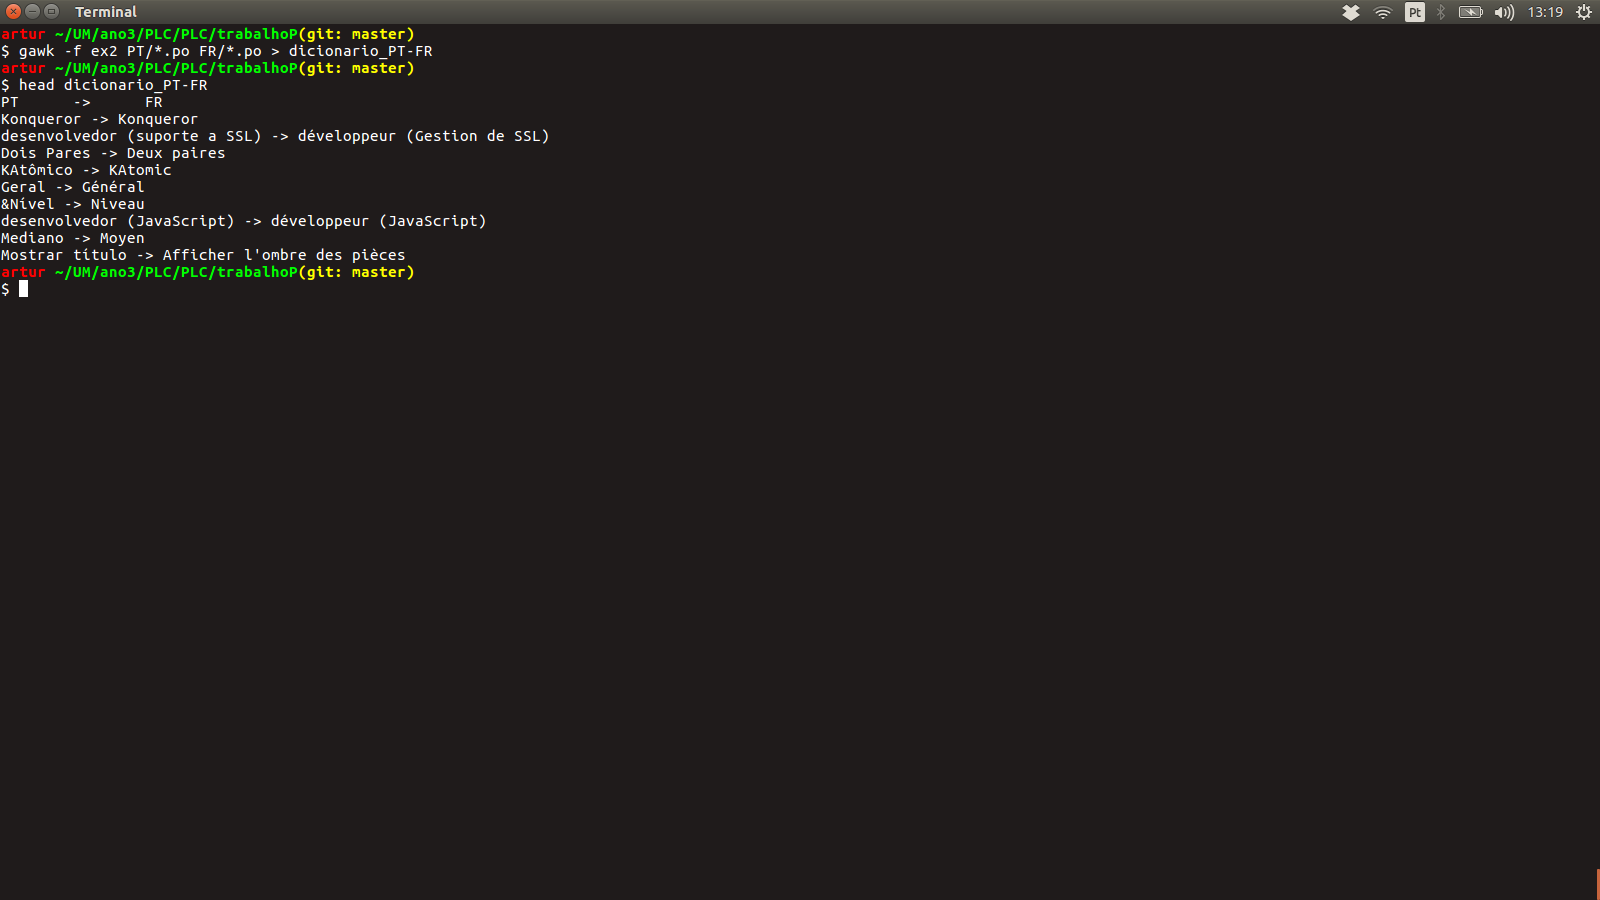
\includegraphics[15,10]{exercicio2.png}
%\caption{Exercicio 2}
%\label{Exercicio 2}
%\end{figure}

%\begin{figure}[h]
%\centering
%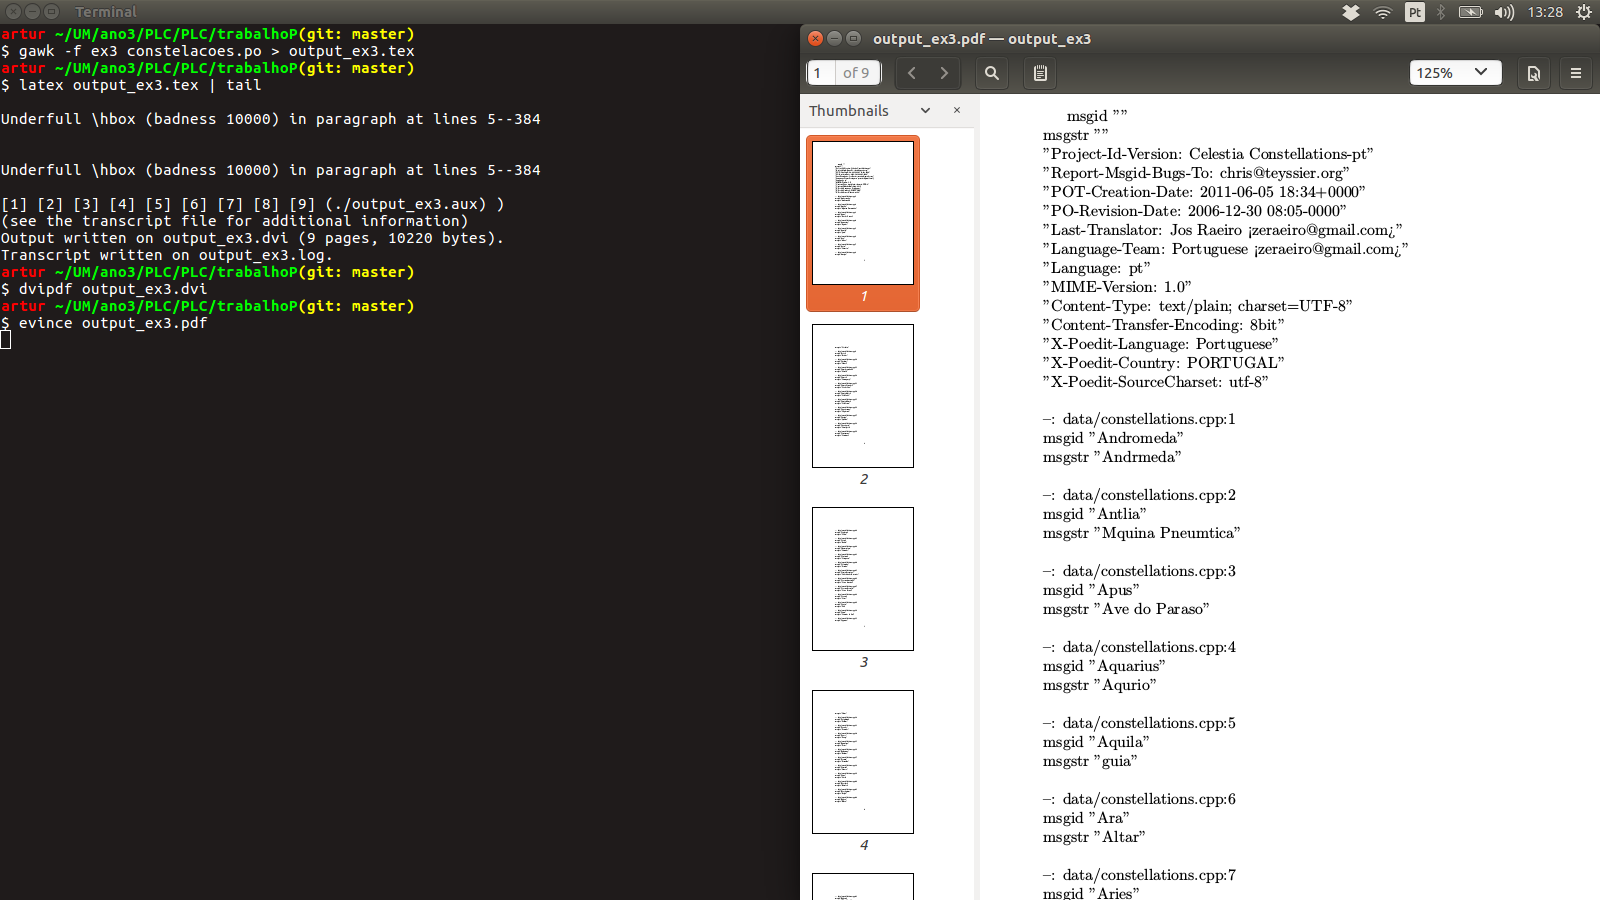
\includegraphics{exercicio3.png}
%\caption{Exercicio 3}
%\label{Exercicio 3}
%\end{figure}


\chapter{Conclusão} \label{concl}
Com este trabalho concluimos que as expressões regulares são excelentes auxiliares na procura do que pretendemos em vários ficheiros simultaneamente.
Para além disso, este trabalho permitiu a familiarização com o LaTex, já que até então não era uma ferramenta utilizada regularmente.
Como perspetiva futura, e mencionado anteriormente, sugerimos a alteração dos ficheiros que não estão com o formato correto, de modo a não conterem "lixo" no resultado da nossa procura. Esta opção seria a mais sensata, dado que criar casos especiais para esses ficheiros é um procedimento mais complexo.



%\appendix
\chapter{Código do Programa}

\href{run:/home/user/Desktop/PLC/trabalhoP/ex/}{Script do exercício 2.5 a)}\\
\href{run:/home/user/Desktop/PLC/trabalhoP/ex2/}{Script do exercício 2.5 b)}\\
\href{run:/home/user/Desktop/PLC/trabalhoP/ex3/}{Script do exercício 2.5 c)}\\



\end{document}
